\chapter{The Evolution of Cheating: From Debugging Tools to an Organized Industry}

The history of cheating in video games is deeply intertwined with the evolution of the industry itself. What began as debugging tools for developers gradually transformed into a clandestine culture of modifications, and with the advent of online gaming, an organized and profitable industry with ties to cybercrime \parencite{consalvo2007cheating}. At the same time, the fight against cheating led to the development of \textbf{anti-cheat systems}, which evolved from simple integrity checks to sophisticated solutions incorporating artificial intelligence and deep system access \parencite{yan2005cheats}.

\section{The Early Days: Debugging Tools and Experimental Modifications}

Before video games became a mainstream form of entertainment, early cheating emerged as a necessity within software development. In the 1970s and 1980s, developers embedded debugging tools within their games to facilitate testing. These systems allowed programmers to modify internal values such as lives, ammunition, and speed, enabling them to test different scenarios without playing through the entire game \parencite{smith2018konami}.

Some of these tools remained accessible in commercial releases, either unintentionally or as a deliberate choice by developers. This led to the creation of the first \textbf{cheat codes}, which were key combinations or commands that altered gameplay. One of the most iconic examples is the \textbf{Konami Code} (↑ ↑ ↓ ↓ ← → ← → B A), introduced in \textit{Gradius} (1986) and later popularized in \textit{Contra} (1988) \parencite{kent2001ultimate}. While these codes were not designed to affect competition, they set a precedent for the intentional modification of gameplay.

\section{The Rise of Cheating in Consoles and PC}

As the video game industry grew throughout the 1980s and 1990s, cheating expanded beyond debugging tools and built-in cheat codes. With the advent of home consoles, external devices specifically designed to modify gameplay began to appear.

\subsection{Cheat Devices: Game Genie, GameShark, and Pro Action Replay}

The first dedicated cheat devices were \textbf{modification cartridges}, such as the \textbf{Game Genie} (1990) and the \textbf{GameShark} (1995). These hardware add-ons allowed players to inject custom modifications into a game’s memory, altering key parameters such as health, ammunition, and physics \parencite{supercade2001}. While initially marketed as harmless tools for enhancing single-player experiences, they introduced the concept of \textbf{real-time game manipulation}, which would later be adapted for online environments.

On the PC side, the introduction of \textbf{memory editors} provided users with a more flexible and powerful way to modify game values at runtime. Early programs like \textbf{Cheat Engine} (2000) enabled players to search for specific in-game variables and alter them directly, bypassing the limitations of built-in cheat codes \parencite{gamersatwork2012}. This shift from \textbf{developer-sanctioned cheats} to \textbf{unauthorized external modifications} laid the foundation for more advanced game-hacking techniques.

As gaming technology evolved, so did the tools available for modifying game memory structures. More sophisticated programs such as \textbf{ReClass.NET} emerged, allowing users to analyze and modify game memory at a structural level. Unlike traditional memory scanners, ReClass.NET enables users to reverse-engineer game memory layouts by dynamically inspecting class structures and data offsets in real time \parencite{wang2015reclass}. This advancement significantly improved the ability of cheat developers to create complex modifications, ranging from automatic aimbots to more intricate exploits that manipulate how game logic processes data.

\begin{figure}[h!]
    \centering
    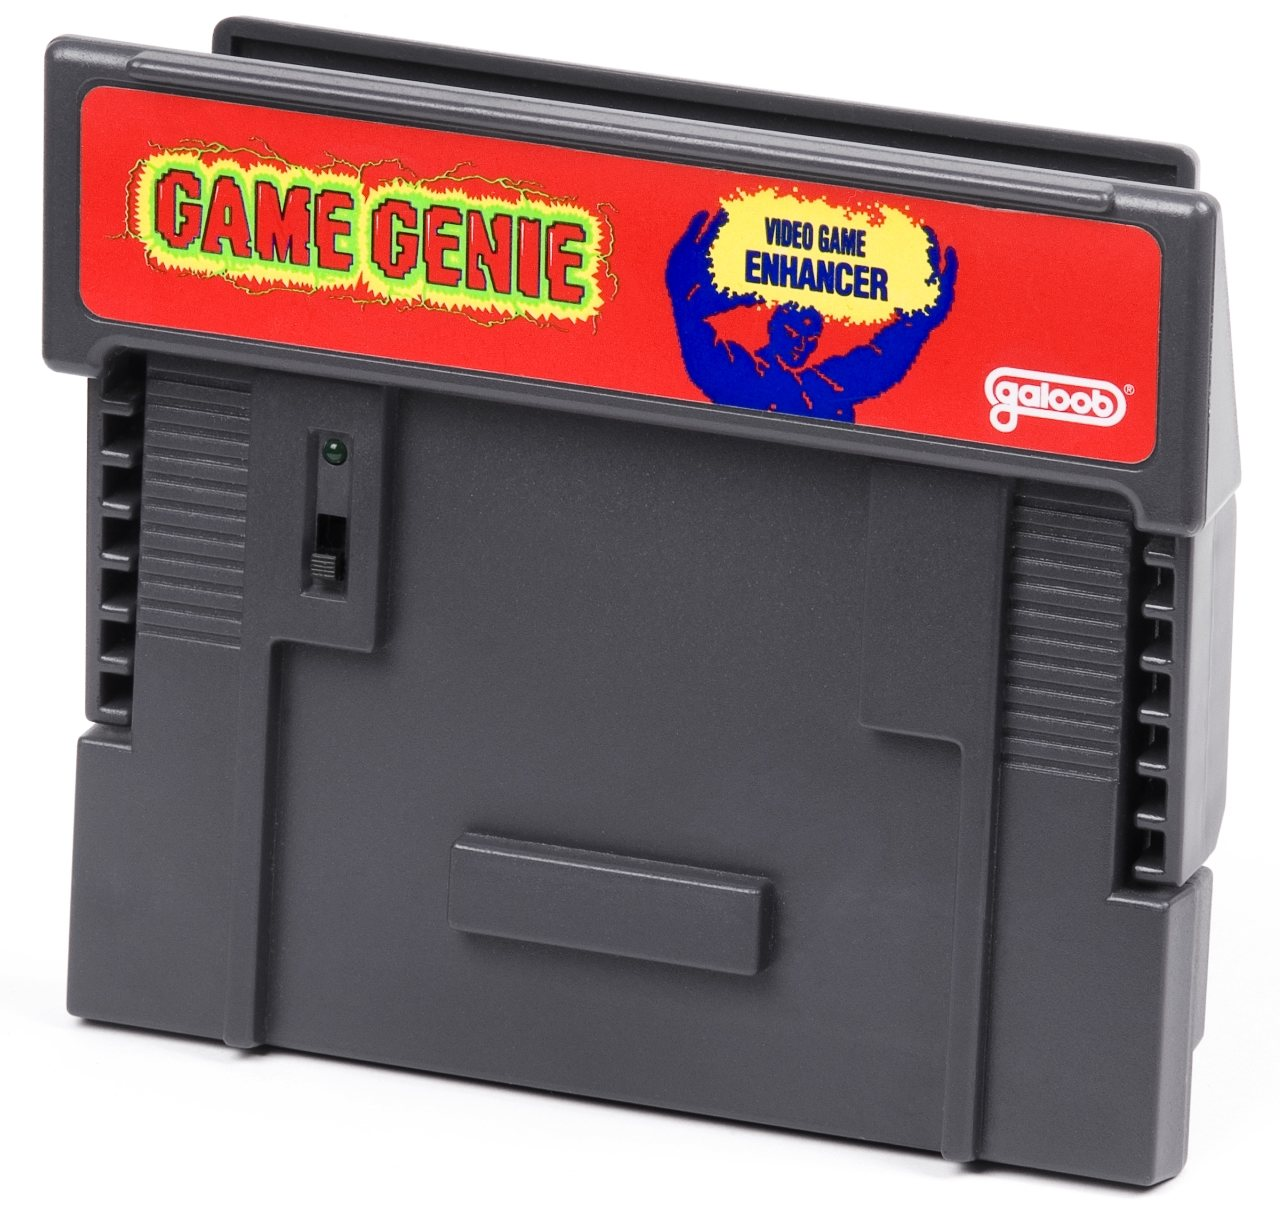
\includegraphics[width=0.5\linewidth]{images/logo-12.jpg}
    \caption{Game Genie}
    \label{fig:enter-label}
\end{figure}

\newpage
These tools, originally designed for educational and debugging purposes, soon became widely used in cheat development, particularly in online gaming environments. As their complexity increased, anti-cheat systems had to adapt rapidly, resulting in an ongoing technological competition between cheat developers and security teams.

\section{The Transition to Online Gaming: Cheating Becomes a Competitive Threat}

The rise of online multiplayer gaming in the late 1990s and early 2000s fundamentally changed the impact of cheating. Unlike single-player cheats, which only affected the individual experience, online cheating directly disrupted fair competition \parencite{yan2005cheats}. As games like \textbf{Quake} (1996), \textbf{Counter-Strike} (1999), and \textbf{Diablo II} (2000) introduced matchmaking and ranking systems, the incentive to cheat increased dramatically \parencite{young2016history}.

As competitive integrity gained prominence, developers began to implement more aggressive measures against cheating, resulting in the creation of server-side and client-side anti-cheat mechanisms. However, as anti-cheat solutions became more sophisticated, cheating techniques also advanced, producing a continuous cycle of adaptation between game security teams and cheat developers.

This progression led to the development of the first organized cheat communities, where players and programmers shared exploits, scripts, and modified game clients. It also marked the beginning of a persistent competition between cheat developers and game security teams, as new forms of cheating emerged alongside increasingly complex anti-cheat measures.

\section{The Birth and Evolution of Anti-Cheat Systems}

As online gaming became increasingly competitive, the integrity of fair play was challenged by the widespread use of cheats. Unlike single-player modifications, which had no broader consequences, cheating in multiplayer environments compromised \textbf{matchmaking, rankings, and esports competitions}, creating frustration among players and damaging the credibility of competitive gaming. 

Early attempts to mitigate cheating relied on \textbf{server-side validation}, where game servers monitored player actions for anomalies that suggested external manipulation. These checks aimed to detect unnatural behavior, such as \textbf{impossible movement speeds, improbable accuracy, and modifications to game assets} that altered visibility constraints. However, this approach had significant limitations, as many cheats operated entirely on the \textbf{client side}, modifying game data before it was transmitted to the server. As a result, more sophisticated \textbf{client-side anti-cheat solutions} were developed to monitor and detect unauthorized modifications directly within the player’s system.

One of the first dedicated anti-cheat programs was \textbf{PunkBuster}, developed by Even Balance, Inc. and introduced in \textbf{2000}. Initially implemented in \textit{Return to Castle Wolfenstein} and later in \textit{Battlefield 1942}, PunkBuster marked a shift from basic server-side detection to \textbf{active client-side monitoring}. It worked by scanning a player’s system for \textbf{known cheat signatures}, verifying \textbf{game file integrity}, and capturing periodic \textbf{in-game screenshots} to identify visual modifications such as \textbf{wallhacks}. Additionally, PunkBuster maintained a \textbf{global ban list}, preventing known cheaters from accessing protected servers. Despite these advancements, \textbf{cheat developers quickly adapted} by employing techniques such as \textbf{code obfuscation}, allowing their software to remain undetected. PunkBuster also faced criticism for its \textbf{aggressive scanning approach}, which occasionally resulted in \textbf{false positives}, banning legitimate players due to conflicts with background applications.

In \textbf{2002}, Valve introduced \textbf{Valve Anti-Cheat (VAC)} alongside \textit{Counter-Strike 1.6}, implementing a more \textbf{automated and data-driven approach} to cheat detection. Unlike PunkBuster, which \textbf{immediately expelled} suspected cheaters, VAC introduced a \textbf{delayed banning system}. This strategy allowed suspected cheaters to continue playing while logging their infractions, making it harder for cheat developers to \textbf{identify detection triggers} and modify their cheats accordingly. In addition to \textbf{signature-based detection}, VAC utilized \textbf{heuristic analysis} to recognize \textbf{abnormal behavioral patterns}, refining its detection algorithms over time. By integrating \textbf{server-side validation} with \textbf{machine learning techniques}, VAC continuously improved its ability to detect and counteract evolving cheats. However, since it \textbf{operated at the user level} rather than the \textbf{kernel level}, advanced cheats that manipulated system memory with higher privileges could still \textbf{bypass its protections}.

As cheat developers refined their evasion techniques, more aggressive anti-cheat solutions emerged. One of the most notable advancements was \textbf{BattleEye}, introduced in 2004 and later adopted in games such as \textit{Arma 2}, \textit{Rainbow Six Siege}, and \textit{PUBG}. Unlike VAC, which prioritized passive detection, BattleEye enforced stricter security measures by running with elevated system privileges. By operating at the kernel level, it could detect and block cheat software that manipulated game memory at a deeper level, making it significantly harder for external programs to alter in-game data without detection. This approach enabled BattleEye to intercept and prevent unauthorized modifications before they could affect gameplay, providing a more proactive defense against sophisticated cheats.

As competitive gaming and esports continued to grow, Riot Games introduced a new anti-cheat solution, Vanguard, designed specifically for \textit{Valorant}. Released in 2020, Vanguard elevated anti-cheat enforcement by implementing persistent kernel-level monitoring. This system actively runs as a background process from the moment the operating system starts, enabling it to detect and prevent unauthorized modifications at the lowest levels of system memory. While this approach is one of the most invasive and effective anti-cheat solutions, its intrusive nature sparked controversy among players concerned about privacy, as the software maintains continuous access to system processes even when the game is not running.

The evolution of anti-cheat systems reflects a continuous technological competition between cheat developers and game security teams. While early efforts relied on rudimentary server-side validation, modern solutions integrate behavioral analysis, machine learning, and kernel-level access to provide more robust protection. Despite these advancements, cheat developers continually adapt, ensuring that no anti-cheat system remains impenetrable for long. This dynamic perpetuates an ongoing cycle of exploitation and countermeasures in the digital landscape of competitive gaming.

This historical evolution has given rise to a wide variety of anti-cheat implementations, each shaped by the needs and challenges of its era.

The continuous development of anti-cheat solutions over the past two decades can be summarized through a timeline of key technologies. Figure~\ref{fig:timeline-anticheat-balanced} provides a chronological overview of the most influential anti-cheat systems, from early client-side detectors to modern kernel-level and behavior-based solutions.

\begin{figure}[h!]
    \centering
    \begin{tikzpicture}[x=0.85cm, y=1cm]
        % Línea del tiempo
        \draw[thick, -{Latex[length=3mm]}] (0,0) -- (16,0);
        \node[below=0.5cm] at (16,0) {\textbf{Year}};

        % Eventos ajustados manualmente (x ≠ año directamente)
        \foreach \x/\year/\label/\ypos in {
            0/2000/PunkBuster/1.6,
            1.5/2001/NProtect\\GameGuard/-1.6,
            3/2002/VAC\\(Valve Anti-Cheat)/1.6,
            4.5/2004/BattleEye/-1.6,
            7/2012/FairFight/1.6,
            10/2018/Easy Anti-Cheat/-1.6,
            12/2020/Vanguard/1.6,
            14.5/2023/VAC Live/-1.6
        } {
            \draw[gray, dashed] (\x,0) -- (\x,\ypos);
            \filldraw[black] (\x,0) circle (2pt);
            \node[align=center, font=\small] at (\x,\ypos) {\label\\(\year)};
        }

        % Marcas de tiempo estilizadas
        \foreach \x/\label in {
            0/2000, 3/2002, 4.5/2004, 7/2012,
            10/2018, 12/2020, 14.5/2023
        } {
            \draw (\x,0.1) -- (\x,-0.1);
            \node[below] at (\x,-0.2) {\label};
        }

    \end{tikzpicture}
    \caption{Chronological overview of key anti-cheat systems introduced between 2000 and 2023.}
    \label{fig:timeline-anticheat-balanced}
\end{figure}

Among the systems depicted in the timeline, several stand out for their unique approach and impact.

nProtect GameGuard, launched in 2001, was among the first anti-cheat solutions to employ rootkit-like behavior. Widely used in Asian MMORPGs, it integrates deeply into the operating system, operating at the kernel level (ring 0), to prevent cheats from interacting with game processes. This deep integration has raised concerns about privacy and system stability \parencite{nprotect_wikipedia}.

FairFight, introduced in 2012, departed from traditional detection mechanisms by using server-side statistical analysis to flag abnormal player behavior. Instead of inspecting memory or processes, it relied on gameplay metrics such as accuracy, reaction time, and movement patterns. This approach made it less intrusive, but also vulnerable to both false positives and high-skill players \parencite{fairfight_website}.

Easy Anti-Cheat (EAC), which gained traction in 2018, became a popular choice for fast-paced competitive games. It combines kernel-level access with performance-friendly design and supports real-time detection of unauthorized drivers, injected DLLs, and tampering attempts, balancing robustness and user transparency \parencite{eac_website}.

Finally, VAC Live, unveiled in 2023, represents Valve's shift toward real-time, data-driven cheat prevention. Unlike the original VAC system, which relied on delayed bans, VAC Live is designed to detect and react to cheats during gameplay. This makes it a critical component in safeguarding the integrity of high-stakes esports matches \parencite{vac_live_announcement}.


\section{The Commercialization of Cheating}

The commercialization of video game cheating has evolved into a multifaceted ecosystem encompassing knowledge-sharing communities, grey-market resellers, and professionalized cheat providers. This transformation reflects a shift from informal exchanges to structured operations with varying degrees of legality and ethical considerations.

Platforms such as \textbf{UnKnoWnCheaTs} serve as non-commercial forums dedicated to the dissemination of information related to game hacking. These communities focus on educational content, including reverse engineering tutorials, memory manipulation techniques, and the release of free cheats contributed by community members. Notably, UnKnoWnCheaTs maintains a strict policy against the sale of cheats, emphasizing its commitment to a non-profit model centered on knowledge exchange \parencite{unknowncheats_forum}.

In contrast, forums like \textbf{ElitePVPers} and \textbf{MPGH} operate as marketplaces where individuals can buy and sell cheats. These platforms facilitate the distribution of paid cheats through various models, including reselling arrangements and subscription-based access. Users often engage in discussions about becoming resellers, highlighting the existence of structured networks for cheat distribution \parencite{elitepvpers_reseller}.

Beyond community forums, a segment of the cheating industry comprises professionalized providers offering sophisticated cheat solutions. These entities develop and sell advanced cheating tools, often featuring capabilities such as kernel-level access, hardware ID spoofing, and real-time updates to circumvent anti-cheat measures. The following table summarizes prominent cheat providers active in the CS2 ecosystem:

\newpage

\begin{table}[h!]
    \centering
    \renewcommand{\arraystretch}{1.4}
    \begin{tabular}{|p{3.2cm}|c|p{4cm}|p{3.8cm}|}
        \hline
        \textbf{Provider} & \textbf{Released} & \textbf{Subscription Price} & \textbf{Access Model} \\
        \hline
        \textbf{Neverlose} \parencite{neverlose2020} & 2020 & €29/month, €69/3 months, €129/year & Invite-only \\
        \hline
        \textbf{Memesense} \parencite{memesense2023} & 2023 & \$4/14 days, \$8/month, \$12/3 months & Public access \\
        \hline
        \textbf{Fatality.win} \parencite{fatality2022} & 2022 & \$33/month & Invite-only \\
        \hline
        \textbf{Project Infinity} \parencite{projectinfinity2017} & 2017 & €14.99/month, €29.99/3 months, €99.99 lifetime & Public access \\
        \hline
        \textbf{Midnight} \parencite{midnight2019} & 2019 & £5.15/month & Public access \\
        \hline
        \textbf{Onetap} \parencite{onetap2024} & 2024 & \$20/month & Public access \\
        \hline
        \textbf{Skeet (Gamesense)} \parencite{skeet2016} & 2016 & \$20/month & Invite-only + HWID locked \\
        \hline
    \end{tabular}
    \caption{Overview of major CS2 cheat providers, including release year, pricing models, and access restrictions.}
    \label{tab:cs2_cheat_providers}
\end{table}


\section*{From Historical Context to Market Impact}

Having explored the historical and sociotechnical evolution of video game cheating, from its inception with debugging tools to its current status as a sophisticated and commercialized industry, we now shift our focus to contemporary market dynamics and their ramifications on gaming communities.

The subsequent chapters will examine the economic structures underpinning the cheating industry, analyzing how monetized cheating services influence player behavior, community trust, and the overall integrity of online gaming environments. Through this analysis, we aim to elucidate the broader social and economic impacts of cheating within the gaming ecosystem.

With the historical framework established, we now proceed to assess the market-driven aspects that perpetuate and shape the landscape of video game cheating.
\newpage



